\section{Appendix}
\label{sec:appendix}

\begin{figure}[H]
  \centering
  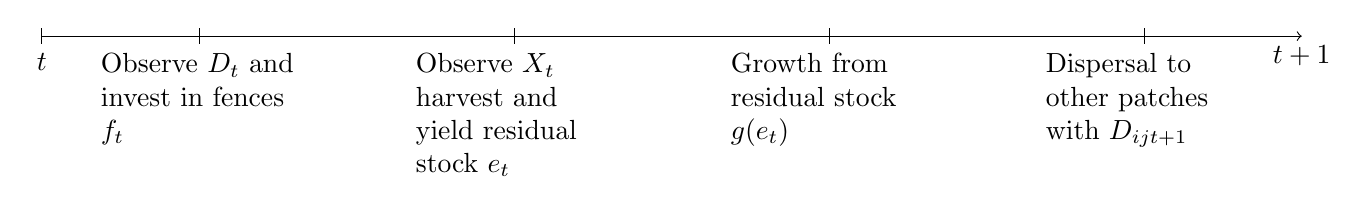
\begin{tikzpicture}
    % Draw the arrow
    \draw[->] (0,0) -- (16,0) node[anchor=north] {$t+1$};
    % Draw ticks and labels
    \draw (0, .1)--(0,-.1) node[anchor = north]{$t$};
    \draw (2, .1)--(2,-.1) node[anchor = north, text width = 2.5cm]{Observe $D_t$ and invest in fences  $f_{t}$};
    \draw (6, .1)--(6,-.1) node[anchor = north, text width = 2.5cm]{Observe $X_t$ harvest and yield residual stock $e_t$};
    \draw (10, .1)--(10,-.1) node[anchor = north, text width = 2.5cm]{Growth from residual stock $g(e_t)$};
    \draw (14,.1)--(14,-.1) node[anchor = north, text width = 2.5cm]{Dispersal to other patches with $D_{ijt+1}$};
  \end{tikzpicture}
  \caption{Timing of the model}
  \label{fig:timing}
\end{figure}

\newpage


\subsection{Proofs}

\subsubsection{Proof of concavity}

Starting from the first order conditions in equations \ref{eq:foc_control_non_cooperative} and \ref{eq:foc_fence_non_cooperative} and omitting time subscripts in $t$ (but remaining in $t+1$), the second order derivatives are :

\begin{align}
\frac{\partial^2 C_i}{\partial e_i^2} &= -c_i'(e_i) + k'_i(e_i) +\delta\left[g_i''(e_i)(1-d_{ij}(f_i, f_j))c_i(X_{it+1}) + \left(g'_i(e_i)(1- d_{ij}(f_i, f_j))\right)^2 c'_i(X_{it+1})\right]\\
%
\frac{\partial^2 C_i}{\partial f_i^2} &= \gamma_i'(f_i) + \delta \left[g_i(e_i)\left(-\frac{\partial d_{ij}}{\partial f_i}c_i'(X_{it+1}) - \frac{\partial^2 d_{ij}}{\partial f_i^2}c_i(X_{it+1}) \right) + g_j(e_j)\left(\frac{\partial d_{ji}}{\partial f_i}c_i'(X_{it+1} + \frac{\partial ^2 d_{ji}}{\partial f_i^2}c_i(X_{it+1})\right) \right]\\
%
\frac{\partial^2 C_i}{\partial e_i \partial f_i} &= \delta g_i'(e_i)\left[-\frac{\partial d_{ij}}{\partial f_i}\left(c_i(X_{it+1}) + c_i'(X_{it+1})g_i(e_i)\right) + c_i(X_{it+1}) \frac{\partial d_{ji}}{\partial f_i}g_j(e_j)\right]\\
%
\frac{\partial ^2 C_i}{\partial f_i \partial e_i} &= -\frac{\partial d_{ij}}{\partial f_i}\delta g_i'(e_i)\left[c_i(X_{it+1}) + g_i(e_i)c_i'(X_{it+1})(1 - d_{ij}(f_i, f_j) \right]
\end{align}

\clearpage
{\footnotesize
\bibliography{bib_fences}
}
\cleardoublepage